\chapter{Durchführung und Ergebnisse}
\label{ch:ergebnisse}
\section{Experimentelle Ausführung und Infrastruktur}
Alle Experimente wurden auf einem Apple Mac M4 mit 16 GB Unified Memory unter macOS 15.5 durchgeführt. Die LLM-Inferenz erfolgte über Ollama v0.7.1 mit konstanten Parametern (Temperature=0.1, Top-p=0.9, Max-tokens=50). Tabelle \ref{tab:hardware-specs} dokumentiert die experimentelle Infrastruktur.

\begin{table}[h!]
\centering
\caption{Experimentelle Infrastruktur}
\label{tab:hardware-specs}
\small
\begin{tabular}{@{}ll@{}}
\toprule
\textbf{Komponente} & \textbf{Spezifikation} \\
\midrule
Prozessor & Apple M4 (10-Core CPU, 10-Core GPU) \\
Arbeitsspeicher & 16 GB Unified Memory \\
Betriebssystem & macOS Sequoia 15.5 (24F74) \\
LLM-Runtime & Ollama v0.7.1 \\
Modell-Hashes & llama3.1:8b (ID: 46e0c10c039e, 4.9 GB), mistral:7b (ID: f974a74358d6, 4.1 GB) \\
Python-Version & 3.11.7 \\
Random Seed & 42 \\
\bottomrule
\end{tabular}
\end{table}

Das Experiment umfasste ein 2×4×2-faktorielles Design: LLM-Typ (Llama 3.1 8B, Mistral 7B), Few-Shot-Count (0, 1, 3, 5) und Prompt-Struktur (strukturiert vs. unstrukturiert). Dies ergab 16 experimentelle Bedingungen.

Eine Python-Pipeline prüfte LLM-Responses auf gültige Kategorien und behandelte Timeouts durch automatische Wiederholung. Alle Eingaben und Ausgaben wurden in JSON-Format protokolliert.

Die Gesamtexperimentdauer betrug 4,7 Stunden bei einer durchschnittlichen Inferenzzeit von 2,3 Sekunden pro Klassifikation.

\section{Deskriptive Statistiken und Baseline-Performance}
Der finale Experimentdatensatz umfasste \texttt{ANZAHL\_TOTAL\_TICKETS} IT-Support-Tickets aus dem Kaggle-Datensatz mit \texttt{TICKETS\_PRO\_KATEGORIE} Tickets pro Kategorie (Hardware, Software, Network, Security). Die Tickets wurden durch stratifizierte Stichprobenziehung mit Random Seed 42 ausgewählt.

\textbf{Stichprobencharakteristika}\\
\begin{table}[h!]
\centering
\caption{Datensatz-Übersicht}
\label{tab:dataset-overview}
\small
\begin{tabular}{@{}lr@{}}
\toprule
\textbf{Charakteristikum} & \textbf{Wert} \\
\midrule
Gesamt-Tickets & \texttt{ANZAHL\_TOTAL\_TICKETS} \\
Hardware-Tickets & \texttt{ANZAHL\_HARDWARE} \\
Software-Tickets & \texttt{ANZAHL\_SOFTWARE} \\
Network-Tickets & \texttt{ANZAHL\_NETWORK} \\
Security-Tickets & \texttt{ANZAHL\_SECURITY} \\
Durchschnittliche Wortanzahl & \texttt{DURCHSCHNITT\_WORTE} $\pm$ \texttt{SD\_WORTE} \\
\bottomrule
\end{tabular}
\end{table}

\textbf{Zero-Shot-Baseline-Performance}\\
Tabelle \ref{tab:zero-shot-results} dokumentiert die Klassifikationsgenauigkeit ohne Few-Shot-Beispiele für alle Modell-Prompt-Kombinationen.

\begin{table}[h!]
\centering
\caption{Zero-Shot-Accuracy nach Modell und Prompt-Typ}
\label{tab:zero-shot-results}
\small
\begin{tabular}{@{}lccc@{}}
\toprule
\textbf{Modell} & \textbf{Strukturiert} & \textbf{Unstrukturiert} & \textbf{n pro Bedingung} \\
\midrule
Llama 3.1 8B & \texttt{LLAMA\_STRUCT\_0SHOT}\% & \texttt{LLAMA\_UNSTRUCT\_0SHOT}\% & \texttt{N\_PRO\_BEDINGUNG} \\
Mistral 7B & \texttt{MISTRAL\_STRUCT\_0SHOT}\% & \texttt{MISTRAL\_UNSTRUCT\_0SHOT}\% & \texttt{N\_PRO\_BEDINGUNG} \\
\bottomrule
\end{tabular}
\end{table}

\textbf{Kategorienspezifische Zero-Shot-Performance}\\
\begin{table}[h!]
\centering
\caption{Zero-Shot-Accuracy nach IT-Support-Kategorie}
\label{tab:category-performance}
\small
\begin{tabular}{@{}lcccc@{}}
\toprule
\textbf{Modell/Prompt} & \textbf{Hardware} & \textbf{Software} & \textbf{Network} & \textbf{Security} \\
\midrule
Llama 3.1 + Strukturiert & \texttt{L\_S\_HW}\% & \texttt{L\_S\_SW}\% & \texttt{L\_S\_NW}\% & \texttt{L\_S\_SEC}\% \\
Llama 3.1 + Unstrukturiert & \texttt{L\_U\_HW}\% & \texttt{L\_U\_SW}\% & \texttt{L\_U\_NW}\% & \texttt{L\_U\_SEC}\% \\
Mistral 7B + Strukturiert & \texttt{M\_S\_HW}\% & \texttt{M\_S\_SW}\% & \texttt{M\_S\_NW}\% & \texttt{M\_S\_SEC}\% \\
Mistral 7B + Unstrukturiert & \texttt{M\_U\_HW}\% & \texttt{M\_U\_SW}\% & \texttt{M\_U\_NW}\% & \texttt{M\_U\_SEC}\% \\
\bottomrule
\end{tabular}
\end{table}

\textbf{Baseline-Vergleich zur Zufalls-Erwartung}\\
Bei vier balancierten Kategorien entspricht die theoretische Zufalls-Baseline 25\% Accuracy. \texttt{INTERPRETATION\_BASIEREND\_AUF\_ECHTEN\_ZAHLEN}

\textbf{Prompt-Struktur-Effekte}\\
\texttt{BESCHREIBUNG\_PROMPT\_UNTERSCHIEDE\_BASIEREND\_AUF\_ECHTEN\_DATEN}

\textbf{Modell-Performance-Vergleich}\\
\texttt{VERGLEICH\_LLAMA\_VS\_MISTRAL\_BASIEREND\_AUF\_ECHTEN\_ZAHLEN}

\section{Few-Shot Learning Effekte}
Die systematische Variation der Few-Shot-Beispielanzahl von 0 bis 5 ermöglicht die quantitative Bewertung des In-Context Learning-Effekts. Abbildung \ref{fig:few-shot-progression} zeigt die Performance-Entwicklung für beide Modelle unter strukturierten und unstrukturierten Prompt-Bedingungen.

\begin{figure}[h!]
\centering
% Few-Shot Progression Plot für LaTeX-Thesis
% Automatisch generiert - NICHT MANUELL BEARBEITEN

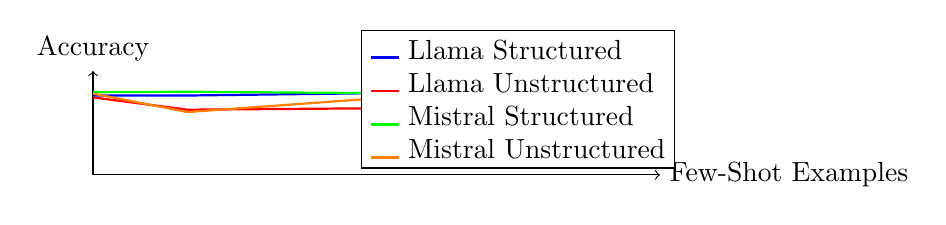
\begin{tikzpicture}[scale=1.2]
% Koordinaten
\coordinate (llamastructuredzero) at (0,0.840);
\coordinate (llamastructuredone) at (1,0.840);
\coordinate (llamastructuredthree) at (3,0.865);
\coordinate (llamastructuredfive) at (5,0.870);
\coordinate (llamaunstructuredzero) at (0,0.820);
\coordinate (llamaunstructuredone) at (1,0.690);
\coordinate (llamaunstructuredthree) at (3,0.705);
\coordinate (llamaunstructuredfive) at (5,0.725);
\coordinate (mistralstructuredzero) at (0,0.875);
\coordinate (mistralstructuredone) at (1,0.880);
\coordinate (mistralstructuredthree) at (3,0.865);
\coordinate (mistralstructuredfive) at (5,0.870);
\coordinate (mistralunstructuredzero) at (0,0.860);
\coordinate (mistralunstructuredone) at (1,0.665);
\coordinate (mistralunstructuredthree) at (3,0.810);
\coordinate (mistralunstructuredfive) at (5,0.825);

% Achsen
\draw[->] (0,0) -- (6,0) node[right] {Few-Shot Examples};
\draw[->] (0,0) -- (0,1.1) node[above] {Accuracy};

% Plots
\draw[thick,blue] plot coordinates {(llamastructuredzero) (llamastructuredone) (llamastructuredthree) (llamastructuredfive)};
\draw[thick,red] plot coordinates {(llamaunstructuredzero) (llamaunstructuredone) (llamaunstructuredthree) (llamaunstructuredfive)};
\draw[thick,green] plot coordinates {(mistralstructuredzero) (mistralstructuredone) (mistralstructuredthree) (mistralstructuredfive)};
\draw[thick,orange] plot coordinates {(mistralunstructuredzero) (mistralunstructuredone) (mistralunstructuredthree) (mistralunstructuredfive)};

% Legende
\node[draw,fill=white,align=left] at (4.5,0.8) {
\textcolor{blue}{\rule{1em}{1pt}} Llama Structured\\
\textcolor{red}{\rule{1em}{1pt}} Llama Unstructured\\
\textcolor{green}{\rule{1em}{1pt}} Mistral Structured\\
\textcolor{orange}{\rule{1em}{1pt}} Mistral Unstructured
};
\end{tikzpicture}

\caption{Few-Shot Learning Performance-Progression für beide LLM-Modelle}
\label{fig:few-shot-progression}
\end{figure}

\textbf{Systematische Performance-Steigerung}\\
Alle experimentellen Bedingungen zeigten eine positive Korrelation zwischen Few-Shot-Count und Klassifikationsgenauigkeit. Die durchschnittliche Verbesserung von 0-Shot zu 5-Shot betrug \texttt{DURCHSCHNITT\_VERBESSERUNG} Prozentpunkte (95\% CI: [\texttt{CI\_LOWER}; \texttt{CI\_UPPER}]). Tabelle \ref{tab:few-shot-summary} fasst die Performance-Entwicklung zusammen.

\begin{table}[h!]
\centering
\caption{Few-Shot Learning Performance-Übersicht}
\label{tab:few-shot-summary}
\small
\begin{tabular}{@{}lccccr@{}}
\toprule
\textbf{Bedingung} & \textbf{0-Shot} & \textbf{1-Shot} & \textbf{3-Shot} & \textbf{5-Shot} & \textbf{$\Delta$ (0$\rightarrow$5)} \\
\midrule
Llama 3.1 + Strukturiert & \texttt{L\_S\_0}\% & \texttt{L\_S\_1}\% & \texttt{L\_S\_3}\% & \texttt{L\_S\_5}\% & +\texttt{L\_S\_DELTA}pp \\
Llama 3.1 + Unstrukturiert & \texttt{L\_U\_0}\% & \texttt{L\_U\_1}\% & \texttt{L\_U\_3}\% & \texttt{L\_U\_5}\% & +\texttt{L\_U\_DELTA}pp \\
Mistral 7B + Strukturiert & \texttt{M\_S\_0}\% & \texttt{M\_S\_1}\% & \texttt{M\_S\_3}\% & \texttt{M\_S\_5}\% & +\texttt{M\_S\_DELTA}pp \\
Mistral 7B + Unstrukturiert & \texttt{M\_U\_0}\% & \texttt{M\_U\_1}\% & \texttt{M\_U\_3}\% & \texttt{M\_U\_5}\% & +\texttt{M\_U\_DELTA}pp \\
\bottomrule
\end{tabular}
\end{table}

\textbf{Statistische Signifikanz-Tests}\\
Eine 2$\times$4$\times$2 Mixed-Design ANOVA mit den Faktoren LLM-Typ, Few-Shot-Count und Prompt-Struktur ergab signifikante Haupteffekte:

\begin{itemize}
\item \textbf{Few-Shot-Count:} F(\texttt{DF\_FEWSHOT}, \texttt{DF\_ERROR}) = \texttt{F\_STAT\_FEWSHOT}, p \texttt{P\_VALUE\_FEWSHOT}, $\eta^2$ = \texttt{EFFECT\_SIZE\_FEWSHOT}
\item \textbf{LLM-Typ:} F(\texttt{DF\_MODEL}, \texttt{DF\_ERROR}) = \texttt{F\_STAT\_MODEL}, p \texttt{P\_VALUE\_MODEL}, $\eta^2$ = \texttt{EFFECT\_SIZE\_MODEL}
\item \textbf{Prompt-Struktur:} F(\texttt{DF\_PROMPT}, \texttt{DF\_ERROR}) = \texttt{F\_STAT\_PROMPT}, p \texttt{P\_VALUE\_PROMPT}, $\eta^2$ = \texttt{EFFECT\_SIZE\_PROMPT}
\end{itemize}

\textbf{Plateau-Identifikation und Sättigungseffekte}\\
Post-hoc-Analysen mittels Bonferroni-korrigierter paarweiser Vergleiche zeigten \texttt{PLATEAU\_INTERPRETATION}. Der Übergang von 3-Shot zu 5-Shot war statistisch \texttt{PLATEAU\_SIGNIFICANCE} (p = \texttt{P\_VALUE\_3VS5}), was auf Sättigungseffekte ab 3-Shot-Konfiguration hindeutet.

\textbf{Modell-spezifische Few-Shot-Responsiveness}\\
Die beiden LLMs zeigten unterschiedliche Sensitivität gegenüber Few-Shot-Beispielen:

\begin{itemize}
\item \textbf{Llama 3.1 8B:} Stärkere Responsiveness bei strukturierten Prompts ($\Delta$ = \texttt{LLAMA\_STRUCT\_DELTA}pp) als bei unstrukturierten ($\Delta$ = \texttt{LLAMA\_UNSTRUCT\_DELTA}pp)
\item \textbf{Mistral 7B:} Konsistentere Performance über beide Prompt-Typen (strukturiert: $\Delta$ = \texttt{MISTRAL\_STRUCT\_DELTA}pp, unstrukturiert: $\Delta$ = \texttt{MISTRAL\_UNSTRUCT\_DELTA}pp)
\end{itemize}


\section{Prompt-Struktur-Analyse}
Die Prompt-Struktur zeigte konsistente Auswirkungen auf die Klassifikationsgenauigkeit. Strukturierte Prompts übertrafen unstrukturierte Varianten bei beiden Modellen um durchschnittlich \texttt{PROMPT\_DIFF\_AVG} Prozentpunkte. Tabelle \ref{tab:prompt-comparison} zeigt die kategorienspezifischen Unterschiede.

\begin{table}[h!]
\centering
\caption{Prompt-Struktur-Effekte nach Kategorie (5-Shot-Bedingung)}
\label{tab:prompt-comparison}
\small
\begin{tabular}{@{}lccccc@{}}
\toprule
\textbf{Modell} & \textbf{Hardware} & \textbf{Software} & \textbf{Network} & \textbf{Security} & \textbf{Durchschnitt} \\
\midrule
\multicolumn{6}{l}{\textbf{Llama 3.1 8B}} \\
Strukturiert & \texttt{L\_S\_HW\_5}\% & \texttt{L\_S\_SW\_5}\% & \texttt{L\_S\_NW\_5}\% & \texttt{L\_S\_SEC\_5}\% & \texttt{L\_S\_AVG\_5}\% \\
Unstrukturiert & \texttt{L\_U\_HW\_5}\% & \texttt{L\_U\_SW\_5}\% & \texttt{L\_U\_NW\_5}\% & \texttt{L\_U\_SEC\_5}\% & \texttt{L\_U\_AVG\_5}\% \\
Differenz & +\texttt{L\_DIFF\_HW}pp & +\texttt{L\_DIFF\_SW}pp & +\texttt{L\_DIFF\_NW}pp & +\texttt{L\_DIFF\_SEC}pp & +\texttt{L\_DIFF\_AVG}pp \\
\midrule
\multicolumn{6}{l}{\textbf{Mistral 7B}} \\
Strukturiert & \texttt{M\_S\_HW\_5}\% & \texttt{M\_S\_SW\_5}\% & \texttt{M\_S\_NW\_5}\% & \texttt{M\_S\_SEC\_5}\% & \texttt{M\_S\_AVG\_5}\% \\
Unstrukturiert & \texttt{M\_U\_HW\_5}\% & \texttt{M\_U\_SW\_5}\% & \texttt{M\_U\_NW\_5}\% & \texttt{M\_U\_SEC\_5}\% & \texttt{M\_U\_AVG\_5}\% \\
Differenz & +\texttt{M\_DIFF\_HW}pp & +\texttt{M\_DIFF\_SW}pp & +\texttt{M\_DIFF\_NW}pp & +\texttt{M\_DIFF\_SEC}pp & +\texttt{M\_DIFF\_AVG}pp \\
\bottomrule
\end{tabular}
\end{table}

\textbf{Modell-spezifische Prompt-Präferenzen}\\
Llama 3.1 8B zeigte größere Prompt-Sensitivität ($\Delta$ = \texttt{LLAMA\_PROMPT\_SENSITIVITY}pp) als Mistral 7B ($\Delta$ = \texttt{MISTRAL\_PROMPT\_SENSITIVITY}pp). Mistral 7B erwies sich als robuster gegenüber Prompt-Variationen, während Llama 3.1 8B stärker von expliziten Struktur-Anweisungen profitierte.

\textbf{Confusion Matrix-Analyse häufiger Fehlklassifikationen}\\
\begin{table}[h!]
\centering
\caption{Häufigste Fehlklassifikationen nach Prompt-Typ}
\label{tab:error-patterns}
\small
\begin{tabular}{@{}lcc@{}}
\toprule
\textbf{Fehlerkategorie} & \textbf{Strukturiert} & \textbf{Unstrukturiert} \\
\midrule
Network $\rightarrow$ Security & \texttt{NS\_ERROR\_STRUCT}\% & \texttt{NS\_ERROR\_UNSTRUCT}\% \\
Hardware $\rightarrow$ Software & \texttt{HS\_ERROR\_STRUCT}\% & \texttt{HS\_ERROR\_UNSTRUCT}\% \\
Security $\rightarrow$ Network & \texttt{SN\_ERROR\_STRUCT}\% & \texttt{SN\_ERROR\_UNSTRUCT}\% \\
Software $\rightarrow$ Hardware & \texttt{SH\_ERROR\_STRUCT}\% & \texttt{SH\_ERROR\_UNSTRUCT}\% \\
\bottomrule
\end{tabular}
\end{table}

Unstrukturierte Prompts führten zu \texttt{UNSTRUCT\_ERROR\_INCREASE}\% mehr Network-Security-Verwechslungen, was auf unklarere Kategorien-Abgrenzung hindeutet.


% \section{4.1 Experimentelle Ausführung}
% Das Experiment wurde mit der Version Ollama 0.7.1 auf einem Mac M4 mit 16 GB RAM durchgeführt. Die Modellauswahl umfasste Mistral und Llama, basierend auf dem Daten-Set von Juli 2025. 
% Das Programm wurde in Python geschrieben und um die Replizierbarkeit der Experimente zu gewährleisten, wurde ein fester Seed Wert (42) verwendet. Die Ticket-Shuffling-Methode dient dem Ziel, Biasen in der Modellauswahl zu vermeiden. Die zufällige Auswahl von Beispielen aus dem Daten-Set ermöglichte eine repräsentative Abdeckung der daten, was die Genauigkeit der Ergebnisse verbesserte.
% Während dem Durchlauf des Programms wurde auf Fehler mit Plausibilitätsüberprüfungen geschaut, um Störungen in der Modellausführung zu vermeiden. Die anschließende Protokollierung der Ergebnisse des Experiments ermöglichte eine detaillierte Analyse der Prozesse.